\documentclass[aspectratio=169,11pt]{beamer}

\usetheme{Madrid}
\usecolortheme{default}

% Colors: Army Black + Gold
\definecolor{armyblack}{RGB}{0,0,0}
\definecolor{armygold}{RGB}{181,152,91}
\definecolor{darkgray}{RGB}{64,64,64}
\definecolor{lightgray}{RGB}{240,240,240}
\definecolor{fcblue}{RGB}{70,130,180}
\definecolor{fcgreen}{RGB}{60,140,60}
\definecolor{fcred}{RGB}{180,60,60}

\setbeamercolor{palette primary}{bg=armyblack,fg=white}
\setbeamercolor{palette secondary}{bg=armygold,fg=armyblack}
\setbeamercolor{palette tertiary}{bg=armyblack,fg=white}
\setbeamercolor{structure}{fg=armyblack}
\setbeamercolor{title}{fg=white}
\setbeamercolor{subtitle}{fg=armygold}
\setbeamercolor{author}{fg=white}
\setbeamercolor{institute}{fg=darkgray}
\setbeamercolor{date}{fg=darkgray}
\setbeamercolor{frametitle}{bg=armyblack,fg=white}
\setbeamercolor{block title}{bg=armygold,fg=armyblack}
\setbeamercolor{block body}{bg=lightgray,fg=armyblack}
\setbeamercolor{item}{fg=armygold}

\setbeamerfont{title}{series=\bfseries,size=\Large}
\setbeamerfont{frametitle}{series=\bfseries}
\setbeamerfont{institute}{size=\normalsize}
\setbeamerfont{date}{size=\normalsize}
\setbeamertemplate{navigation symbols}{}

\hyphenpenalty=10000
\exhyphenpenalty=10000

\usepackage{booktabs}
\usepackage{array}
\usepackage{graphicx}
\usepackage{tikz}
\usetikzlibrary{shapes,arrows.meta,positioning,calc}
\usepackage{hyperref}
\usepackage{tabularx}
\usepackage{colortbl}
\usepackage{fancyvrb}

\hypersetup{colorlinks=true,urlcolor=fcblue}

\setbeamertemplate{footline}{
  \leavevmode%
  \hbox{%
    \begin{beamercolorbox}[wd=.333\paperwidth,ht=2.25ex,dp=1ex,center]{palette primary}%
      \usebeamerfont{author in head/foot}\insertshortauthor
    \end{beamercolorbox}%
    \begin{beamercolorbox}[wd=.334\paperwidth,ht=2.25ex,dp=1ex,center]{palette secondary}%
      \usebeamerfont{title in head/foot}\insertshorttitle
    \end{beamercolorbox}%
    \begin{beamercolorbox}[wd=.333\paperwidth,ht=2.25ex,dp=1ex,right]{palette primary}%
      \insertframenumber{} / \inserttotalframenumber\hspace*{2ex}
    \end{beamercolorbox}}%
  \vskip0pt%
}

\newcommand{\link}[2]{\href{#1}{\footnotesize\texttt{#2}}}

\title[Agents for Research]{Agents for Research}
\subtitle{How to Get the Most Out of Your Agents}
\author[Semmel]{Austin Semmel}
\institute{Department of Mathematical Sciences \\ United States Military Academy}
\date{September 2026}
\titlegraphic{
\includegraphics[height=1.5cm]{Figures/Math_Mule.png}\hspace{1.2cm}
\includegraphics[height=1.5cm]{Figures/qr_agentic.png}\\[2pt]{\tiny\texttt{austinsemmel.com/agentic}}}

\begin{document}

{
\setbeamertemplate{footline}{}
\begin{frame}[noframenumbering]
\titlepage
\end{frame}
}

%==========================================================================
% SLIDE 2: WHAT AN AGENT IS
%==========================================================================
\begin{frame}{An agent takes steps toward your goal}

\begin{columns}[T]
\begin{column}{0.46\textwidth}
\small
Think of a teammate who already has your project open. You bring the intent and the
direction; it handles the execution, \textbf{right in your files.}

\vspace{0.6em}
\begin{itemize}\small
  \item \textbf{Reads} your files to gather its own context
  \item \textbf{Runs} your code and debugs it to meet your intent
  \item \textbf{Fetches}: downloads, searches, web APIs on your behalf
  \item \textbf{Touches only} what you give it permission to touch
  \item \textbf{Can loop} until the job is done\\
        {\scriptsize\texttt{/goal} \textit{run all five models overnight; check every 30 minutes}}
\end{itemize}


\end{column}

\begin{column}{0.52\textwidth}
\centering
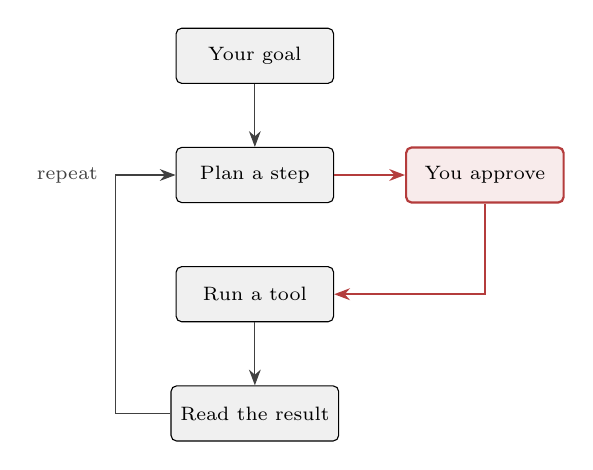
\begin{tikzpicture}[node distance=0.8cm and 0.9cm,
    box/.style={draw=armyblack,fill=lightgray,rounded corners=2pt,
                minimum width=2.0cm,minimum height=0.7cm,font=\scriptsize},
    gate/.style={draw=fcred,thick,fill=fcred!10,rounded corners=2pt,
                minimum width=2.0cm,minimum height=0.7cm,font=\scriptsize},
    arr/.style={-{Stealth[length=2mm]},draw=darkgray}]

  \node[box] (goal) {Your goal};
  \node[box,below=of goal] (plan) {Plan a step};
  \node[gate,right=of plan] (human) {You approve};
  \node[box,below=of plan] (act)  {Run a tool};
  \node[box,below=of act]  (obs)  {Read the result};

  \draw[arr] (goal) -- (plan);
  \draw[arr,fcred,thick] (plan) -- (human);
  \draw[arr,fcred,thick] (human.south) |- (act.east);
  \draw[arr] (act)  -- (obs);
  \draw[arr] (obs.west) -- ++(-0.7,0) |- (plan.west)
        node[midway,left,font=\scriptsize,text=darkgray,xshift=-0.1cm] {repeat};
\end{tikzpicture}
\end{column}
\end{columns}

\vspace{0.4em}
\link{https://docs.claude.com/en/docs/claude-code}{docs.claude.com/en/docs/claude-code}
\end{frame}

%==========================================================================
% SLIDE 3: LITERATURE REVIEW
%==========================================================================
\begin{frame}{How to run an agentic literature review}

This automates the worst part of a literature review: the endless search through
papers that \textit{might} fit your inclusion criteria but turn out to be no practical
use to you.

\vspace{0.3em}
\begin{center}
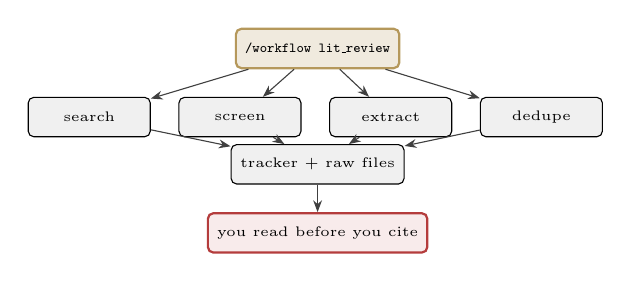
\begin{tikzpicture}[node distance=0.25cm and 0.35cm,
    n/.style={draw=armyblack,fill=lightgray,rounded corners=2pt,minimum width=1.55cm,minimum height=0.5cm,font=\tiny},
    c/.style={draw=armygold,thick,fill=armygold!20,rounded corners=2pt,minimum height=0.5cm,font=\tiny\ttfamily},
    k/.style={draw=fcred,thick,fill=fcred!10,rounded corners=2pt,minimum height=0.5cm,font=\tiny},
    a/.style={-{Stealth[length=1.5mm]},draw=darkgray}]
  \node[c] (cmd) {/workflow lit\_review};
  \node[n,below=0.35cm of cmd,xshift=-2.9cm] (w1) {search};
  \node[n,right=of w1] (w2) {screen};
  \node[n,right=of w2] (w3) {extract};
  \node[n,right=of w3] (w4) {dedupe};
  \node[n,below=0.95cm of cmd] (mrg) {tracker + raw files};
  \node[k,below=0.35cm of mrg] (chk) {you read before you cite};
  \foreach \w in {w1,w2,w3,w4}{\draw[a] (cmd) -- (\w); \draw[a] (\w) -- (mrg);}
  \draw[a] (mrg) -- (chk);
\end{tikzpicture}
\end{center}

\vspace{0.2em}
\begin{columns}[T]
\begin{column}{0.48\textwidth}
\begin{block}{\small Give it to the agents}
\begin{itemize}\scriptsize
  \item Search, retrieve, deduplicate
  \item Screen abstracts against your criteria
  \item Extract methods and results into one table
\end{itemize}
\end{block}
\end{column}
\begin{column}{0.48\textwidth}
\begin{block}{\small Still your responsibility}
\begin{itemize}\scriptsize
  \item Article content, and what you cite it for
  \item Is the gap real, or did your search miss it?
  \item Page numbers and sections for every citation
\end{itemize}
\end{block}
\end{column}
\end{columns}

\end{frame}

%==========================================================================
% SLIDE 4: CITATIONS + CROSSREF
%==========================================================================
\begin{frame}[fragile]{Automate bib citations (then verify them)}

{\small Agents are great at BibTeX. Careful! Sometimes they make mistakes!}

\vspace{0.4em}
\begin{columns}[T]
\begin{column}{0.40\textwidth}
{\scriptsize
\begin{tabular}{@{}ll@{}}
\toprule
\textbf{Key} & \textbf{Claimed} \\
\midrule
Sherbrooke1968 & Oper.\ Res.\ 16 \\
Verhoeff2015 & Transp.\ Res.\ Proc.\ 10 \\
\rowcolor{fcred!12} Cho2017 & Comp.\ \& Ind.\ Eng.\ 109 \\
Hardle2004 & Econometric Th.\ 20 \\
\bottomrule
\end{tabular}}

\vspace{0.7em}
\begin{center}
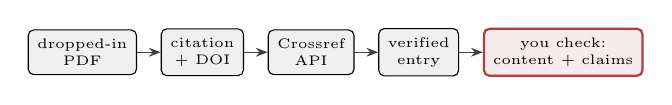
\begin{tikzpicture}[node distance=0.3cm,
    n/.style={draw=armyblack,fill=lightgray,rounded corners=2pt,minimum height=0.55cm,font=\tiny,align=center},
    k/.style={draw=fcred,thick,fill=fcred!10,rounded corners=2pt,minimum height=0.55cm,font=\tiny,align=center},
    a/.style={-{Stealth[length=1.5mm]},draw=darkgray}]
  \node[n] (p) {dropped-in\\PDF};
  \node[n,right=of p] (c) {citation\\+ DOI};
  \node[n,right=of c] (x) {Crossref\\API};
  \node[n,right=of x] (v) {verified\\entry};
  \node[k,right=of v] (h) {you check:\\content + claims};
  \draw[a] (p) -- (c); \draw[a] (c) -- (x); \draw[a] (x) -- (v); \draw[a] (v) -- (h);
\end{tikzpicture}
\end{center}
\end{column}

\begin{column}{0.58\textwidth}
\begin{Verbatim}[fontsize=\scriptsize,frame=single,rulecolor=\color{darkgray}]
$ python3 verify_refs.py

OK   Sherbrooke1968
OK   Verhoeff2015
OK   Hardle2004
FLAG Cho2017
      ! title 39% match
      ! year 2017->2025
      ! vol 109->15
\end{Verbatim}
\end{column}
\end{columns}

\vspace{0.2em}
\link{https://api.crossref.org/works?query.bibliographic=METRIC+multi-echelon+recoverable+item+Sherbrooke}{api.crossref.org/works?query.bibliographic=...}
\end{frame}

%==========================================================================
% SLIDE 5: SKILL FILES
%==========================================================================
\begin{frame}[fragile]{Skill files: repeated prompts and project management}

{\small A skill file does two jobs.}

\vspace{0.4em}
\begin{columns}[T]
\begin{column}{0.50\textwidth}
\begin{block}{\small Repeated prompts}
{\scriptsize One command, the whole routine, the same way every time.}
\end{block}
\begin{Verbatim}[fontsize=\scriptsize,frame=single,rulecolor=\color{darkgray}]
---
name: overleaf_push
description: Sync a local folder with an
  Overleaf project over the Git bridge.
---

MAP=(
    "main.tex               -> ."
    "Figures/*.pdf -> figures"
)

# The token is an internet password in the
# macOS Keychain, read at the moment of use.
# It never lands in a file or a transcript.
\end{Verbatim}
\end{column}
\begin{column}{0.46\textwidth}
\begin{block}{\small Project management}
{\scriptsize A decision log the agent reads first. November picks up where September
stopped.}
\end{block}

\vspace{0.4em}
{\small As a project manager, you determine what context future agents will need to get started: automated session logs + codebase orientation.}
\end{column}
\end{columns}
\end{frame}

%==========================================================================
% SLIDE 7: OVERLEAF / MCP
%==========================================================================
\begin{frame}[fragile]{Automated collaboration}

{\small You and your co-author share one Overleaf project. Pull what they wrote, make
the edit, push it back, open the result.}

\vspace{0.5em}
\begin{columns}[T]
\begin{column}{0.44\textwidth}
\begin{itemize}\small
  \item \textbf{Pull} what your co-author wrote
  \item \textbf{Edit} it locally with the agent
  \item \textbf{Push} it back to their browser
  \item \textbf{Open} the recompiled PDF
\end{itemize}
\vspace{0.4em}
{\small Terminal power, Overleaf ease.}
\vspace{0.4em}

{\scriptsize The plumbing is Overleaf's Git bridge; Model Context Protocol is the same
idea for any outside system.}

\vspace{0.3em}
\begin{center}
\colorbox{white}{\parbox{0.5\linewidth}{\centering\vspace{2pt}
{\color{armyblack}\small\textbf{Hello, World!}}\vspace{2pt}}}\\[2pt]
{\scriptsize\color{armygold}$\downarrow$ one \texttt{/overleaf\_push}}\\[2pt]
\colorbox{white}{\parbox{0.72\linewidth}{\centering\vspace{2pt}
{\color{armyblack}\textbf{Good afternoon, Mathletes!}}\\[3pt]

\includegraphics[width=0.34\linewidth]{Figures/Math_Mule.png}\vspace{2pt}}}
\end{center}
\end{column}
\begin{column}{0.52\textwidth}
\begin{Verbatim}[fontsize=\scriptsize,frame=single,rulecolor=\color{darkgray}]
$ overleaf.sh pull ma376 --apply
pulled main.tex from Overleaf
$ cat main.tex
Hello, World!
$ # the agent makes the edit
-  Hello, World!
+  Good afternoon, Mathletes!
+  \includegraphics{math_mule.png}
$ overleaf.sh push ma376
push ma376: 2 files -> mirror
done. Overleaf is in step.
$ open main.pdf
\end{Verbatim}
\end{column}
\end{columns}

\vspace{0.5em}
\centering
\link{https://modelcontextprotocol.io}{modelcontextprotocol.io}
\hspace{1.5em}
\link{https://www.overleaf.com/learn/how-to/Git_integration}{overleaf.com/learn/how-to/Git\_integration}
\end{frame}

%==========================================================================
% SLIDE 6: WHAT A WORKFLOW IS
%==========================================================================
\begin{frame}{How to incorporate agents into your next project}

{\small One checkpoint per handoff: verify before the next stage builds on it.}

\vspace{0.3em}
\centering
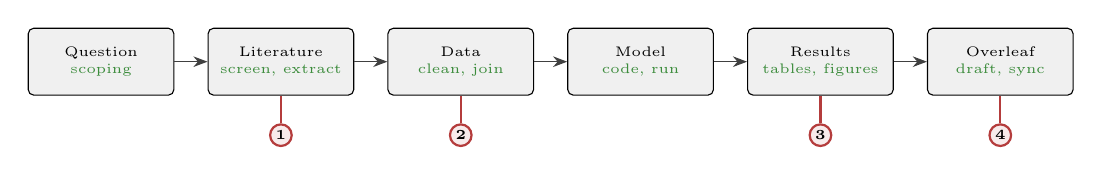
\begin{tikzpicture}[node distance=0.42cm,
    st/.style={draw=armyblack,fill=lightgray,rounded corners=2pt,
               minimum width=1.85cm,minimum height=0.85cm,font=\tiny,align=center},
    gt/.style={draw=fcred,thick,fill=fcred!10,circle,inner sep=1pt,font=\tiny\bfseries},
    arr/.style={-{Stealth[length=1.8mm]},draw=darkgray}]

  \node[st] (q)   {Question\\ \textcolor{fcgreen}{scoping}};
  \node[st,right=of q] (lit) {Literature\\ \textcolor{fcgreen}{screen, extract}};
  \node[st,right=of lit] (dat) {Data\\ \textcolor{fcgreen}{clean, join}};
  \node[st,right=of dat] (mod) {Model\\ \textcolor{fcgreen}{code, run}};
  \node[st,right=of mod] (res) {Results\\ \textcolor{fcgreen}{tables, figures}};
  \node[st,right=of res] (sub) {Overleaf\\ \textcolor{fcgreen}{draft, sync}};

  \foreach \a/\b in {q/lit,lit/dat,dat/mod,mod/res,res/sub}
    \draw[arr] (\a) -- (\b);

  \node[gt,below=0.35cm of lit] (g1) {1};
  \node[gt,below=0.35cm of dat] (g2) {2};
  \node[gt,below=0.35cm of res] (g3) {3};
  \node[gt,below=0.35cm of sub] (g4) {4};
  \foreach \g/\n in {g1/lit,g2/dat,g3/res,g4/sub} \draw[fcred,thick] (\g) -- (\n);
\end{tikzpicture}

\vspace{0.4em}
\begin{columns}[T]
\begin{column}{0.5\textwidth}
{\scriptsize
\textcolor{fcred}{\textbf{1}} Every citation verified against Crossref \\
\textcolor{fcred}{\textbf{2}} Row counts and units checked against the source extract}
\end{column}
\begin{column}{0.5\textwidth}
{\scriptsize
\textcolor{fcred}{\textbf{3}} Numbers reproduce from a script you can rerun \\
\textcolor{fcred}{\textbf{4}} You read the diff before your co-author sees it}
\end{column}
\end{columns}

\vspace{0.4em}
{\scriptsize The agent moves fastest on the green work. The red gates make the
result publishable.}
\end{frame}

%==========================================================================
% SLIDE 8: SO WHAT
%==========================================================================
\begin{frame}{The so what}

\begin{block}{\small What got cheaper}
\begin{itemize}\scriptsize
  \item Screening hundreds of papers down to the thirty that matter
  \item Cleaning and joining data before modeling starts
  \item Turning a finished analysis into tables, figures, and slides
\end{itemize}
\end{block}

\begin{block}{\small What got more expensive}
\begin{itemize}\scriptsize
  \item Anything with your name on it needs verification you can show
  \item A fluent wrong answer hides longer than a clumsy one
  \item Provenance is yours to build in
\end{itemize}
\end{block}

\vspace{0.3em}
{\small Producing a competent draft is now close to free, but your responsibility for
the veracity of the content hasn't changed.}

\vspace{0.3em}
{\scriptsize \textbf{Start here:} docs.claude.com/claude-code ~·~ api.crossref.org ~·~ modelcontextprotocol.io}
\end{frame}

\end{document}
